\section{Verteilte Anwendungen mit Sockets}

Eigenständige \codebf{Client-Server-Anwendungen} können auf 3 verschiedene Arten umgesetzt werden:

\begin{itemize}
    \item Socket-Programmierung (Socket: Schnittstelle für \textbf{UDP} / \textbf{TCP} \footnote{
    UDP: \textit{User Datagram Protocol}; TCP: \textit{Transmission Control Protocol}
    })
    \item \textbf{RMI} \textit{Remote Method Invocation}: Die Methode eines Objektes, das auf einem anderen Rechner liegt, kann von einem anderen entfernten Rechner aufgerufen werden; RMI basiert auf Sockets und stellt somit eine höhere Schnittstelle mit einem höheren Abstraktionsniveau dar
    \item \textbf{indirekte Kommunikation}: Nachrichten werden durch einen Vermittler von einem Sender zu einem Empfänger weitergeleitet
\end{itemize}


\subsection{Schichtenmodell}

\subsection*{Schicht 1 - (Physical Layer)}

Diese Schicht ist zuständig für die Übertragung von Datenblöcken zwischen zwei Rechnern, die direkt miteinander verbunden sind (genauso wie \textbf{Schicht 2}).\\
Sie ist zuständig für die Übertragung einzelner Bits und wird deshalb auch \textbx{Bitübertragungsschicht} genannt.

\subsection*{Schicht 2 - DataLink Layer}

\noindent
Wie Schicht 1 ist auch diese Schicht zuständig für die Übertragung von Datenblöcken zwischen zwei direkt miteinander verbundenen Rechnern.\\

\noindent
Die Schicht hat die Aufgabe, einzelne Bits zu einem Datenblock in einem bestimmten Format zusammenzufassen.\\
$\rightarrow$ bestimmte Informationen wie z.B. Adressen haben eine bestimmte Struktur und Bitlänge und stehen an bestimmten Stellen in einem Datenblock.\\

\noindent
Bei lokalen Netzen wie {bspw.} Ethernet hat die \textbf{Leitungsschicht} durch das gemeinsame Medium noch weitere Funktionen: Sie garantiert, dass immer nur höchstens eine Station sendet, außerdem werden durch sie die angeschlossenen Rechner korrekt adressiert\footnote{
``Bei einer Punkt-zu-Punkt-Leitung kann eine empfangene Station davon ausgehen, dass die ankommenden Daten für sie bestimmt sind, bei einem gemeinsamen Medium dagegen nicht.``~\cite[257]{Oec22}
}.

\begin{tcolorbox}[enlarge top by=0.5cm,enlarge bottom by=0.5cm]
    Schicht 1 und 2 werden über Hardware ({bspw.} Ethernet-Adapter) und entsprechende Treiber im Betriebssystem realisiert.
\end{tcolorbox}

\noindent
Die beiden Funktionen (eine Station sendet, korrekte Adressierung) werden als \textbf{Medium Access Control} (\textit{MAC}) bezeichnet und bilden eine Teilschicht innerhalb der Leitungsschicht (\textit{DataLink Layer}).\\
Die entsprechenden Adressen heißen deshalb \textit{MAC-Adressen}.

\subsection*{Schicht 3}
Schicht 3 ist die \textbf{Vermittlungsschicht} (\textbf{Network Layer}), hier befindet sich das \textbf{IP-Protokoll}, über das Rechner verbunden werden, die an verschiedene Netze mit unterschiedlichen Netztechnologien angeschlossen sind.\\

\noindent
Jeder Netzanschluss enthält eine eindeutige \textbf{IP-Adresse}.\\
Die Schicht sorgt für eine einheitliche, strukturierte und weltweit eindeutige Adressierung (vgl.~\cite[258]{Oec22}).\\

\noindent
Über das IP-Protokoll werden Datenpakete über verschiedene Netze weitergeleitet, bis sie beim Zielrechner ankommen.\\

\noindent
Es kann durchaus vorkommen, dass Datenpakete verlorengehen, oder verzögert und/oder in unterschiedlicher Reihenfolge beim Empfänger eintreffen.

\begin{tcolorbox}[enlarge top by=0.5cm,enlarge bottom by=0.5cm]
    Schicht 3 und 4 sind i.d.R. Teil des Betriebssystemkerns.
\end{tcolorbox}

\subsection*{Schicht 4}
Schicht 4 ergänzt die Adressierung in Schicht 3 um \textit{Kontaktpunkte} durch \textbf{Portnummern}, und wird \textbf{Transportschicht} (\textbf{Transport Layer}) genannt.\\

\noindent
Zwei verbreitete Transportprotokolle sind \textbf{UDP} und \textbf{TCP};

\begin{itemize}
    \item \textbf{UDP} (\textit{User Datagram Protocol}) hat dieselbe Eigenschaften wie das IP-Protokoll und erweitert es um die Adressierung mit Portnummern.\\
    Es ist genauso   \textit{verbindungslos} und \textit{unzuverlässig}\footnote{
    es sind Verluste und Reihenfolgevertauschungen möglich.
    } wie das IP-Protokoll.
    \item \textbf{TCP} (\textit{Transmission Control Protocol}) behebt die Nachteile des IP-Protokolls: Die Empfänger müssen den Nachrichtenerhalt bestätigen\footnote{ ``\textit{ACK}``,
    was wiederum von Sender-Seite überwacht wird; s.a. ``Transmission Control Protocol``: \url{https://en.wikipedia.org/wiki/Transmission_Control_Protocol} - abgerufen 30.01.2024
    }, ansonsten wird die Nachricht nochmals gesendet.
\end{itemize}


\subsection*{Schicht 5}
Schicht 5 ist die \textbf{Anwendungsschicht}\footnote{
    Im Buch werden 5 Schichten aufgeführt, das \textbf{OSI-Modell} hat in der \textit{Anwendungsorientierten Schicht} noch zwei zusätzliche Schichten, die \textbf{Session-Layer} und die \textbf{Presentation-Layer} (\url{https://en.wikipedia.org/wiki/OSI_model} - abgerufen 3.2.2024)
} (\textbf{Application Layer}), in ihr wird die Kommunikation der Anwendung abgewickelt (bspw. \textit{www}, \textit{email}, \textit{Videokonferenzen}).

\begin{tcolorbox}[enlarge top by=0.5cm,enlarge bottom by=0.5cm]
    Schicht 5 wird über Anwendungsprozesse realisiert.
\end{tcolorbox}


\begin{figure}
    \centering
    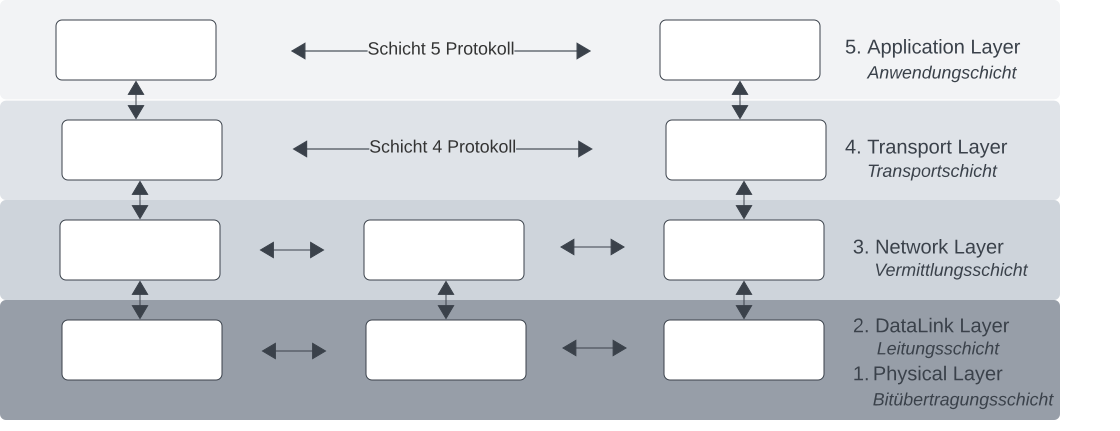
\includegraphics[width=16cm]{chapters/fopt5/img/layers}
    \caption{Skizze des Schichtenmodels. (Quelle: in Anlehnung an \cite[257, Bild 5.2]{Oec22})}
    \label{fig:layers}
\end{figure}


\subsection{IP-Adressen und DNS-Namen}

Ein Rechner kann mehrere Netzanschlüsse haben.\\

\noindent
Jeder dieser Netzanschlüsse ist eine weltweit eindeutige IP-Adresse zugeordnet.\\

\noindent
IP-Adressen können auch durch (Rechner-)Namen aufgelöst werden durch das \textbf{Domain Name System} (\textit{DNS}).\\

\noindent
Ein DNS-Name kann auch mehrere Aliase besitzen; dadurch, dass ein Rechner mehrere IP-Adressen haben kann (bspw. durch mehrere Netzanschlüsse) besteht so zwischen Rechnernamen und IP-Adressen eine $m:n$-Beziehung.


\subsection{Das Transportportprotokoll UDP}

Transportprotokolle existieren, damit mehrere Anwendungen, die über das Internet kommunizieren, gleichzeitig laufen und Daten untereinander austauschen können.\\

\noindent
Bei der Übertragung von Daten besitzt IP die Eigenschaften, dass Daten in unterschiedlicher Reihenfolge eintreffen können, was aus Anwendersicht problematisch ist; auf Anwendungsschicht könnte man hier Gegenmaßnahmen treffen, aber das würde bedeuten, die Gegenmaßnahmen in jeder Anwendung implementieren zu müssen - deshalb werden diese Problematiken in der \textbf{Transportschicht} über \textbf{Transportprotokolle} gelöst.\\

\noindent
\textbf{UDP} (\textbf{User Datagram Protocol}) ermöglicht die Kommunikation verschiedener Dienste gleichzeitig (spezifische Anwendung wird über Portnummer adressiert).\\

\noindent
Ein \textbf{Datagramm}\footnote{
Kunstwort abgeleitet aus\textit{Telegramm} (vgl.~\cite[260]{Oec22})
} bezeichnet eine Dateneinheit, die in ein IP-Paket gepackt und über das Netz verschickt wird.

\begin{tcolorbox}[enlarge top by=0.5cm,enlarge bottom by=0.5cm]
\textbf{UDP} ist Nachrichtenorientiert.
\end{tcolorbox}

\noindent
Ein \textbf{UDP-Datagram} enthält neben der Zielportnummer auch die Quellportnummer, damit der Empfänger dem Sender antworten kann.

\noindent
UDP ist wie IP \textbf{verbindungslos} - es können \textit{Datagrammverluste} oder \textit{Reihenfolgevertauschungen} von Datagrammen vorkommen.\\

\noindent
UDP ist \textbf{datagrammorientiert}: Eine an das UDP-Protokoll übergebene Menge an Daten wird in ein Datagramm gepackt und über IP verschickt\\
$\rightarrow$ die Daten kommen als Einheit beim Empfänger an (entspricht dem Verhalten einer \textbf{Message Queue})


\subsection{Das Transportprotokoll TCP}

\textbf{TCP} ist ein Protokoll für genau zwei Partner, weshalb es nicht mit \textbf{Multicast} genutzt werden kann.\\

\noindent
\textbf{TCP} ist verbindungsorientiert, wobei der Verbindungsauf- und -abbau einen gewissen Aufwand erfordert\footnote{
    Wenn Datenverluste nicht hinnehmbar sind und wegen höherem Aufwand für die Verbindung trotzdem UDP verwendet wird, erweitert man die Anwendung entsprechend um Gegenmaßnahmen für den Datenverlust (vlg. \cite[261]{Oec22}).
}.

\noindent
\textbf{TCP} ist ein zuverlässiges Protokoll, es können keine Daten vertauscht oder verloren gehen, außerdem gibt es eine \textbf{Flusskontrolle} (zum Verhindern einer Überflutung des Empfängers mit Datenpaketen)\footnote{Empfangsbestätigung abwarten} und eine \textbf{Überlastkontrolle} (um eine Überlastung des Netzes zu verhindern)\footnote{informal: falls ein ACK ausbleibt, könnte der Sender versucht sein, ständig neue Pakete hinterherzuschicken, was zu einem Stau führen könnte. Siehe hierzu auch ``Modul 6: TCP-Überlastkontrolle``: \url{https://leischner.inf.h-brs.de/lehre/ikomm/ikomm06-ueberlastkontrolle.pdf} - abgerufen 30.01.2024}.\\

\noindent
\textbf{TCP} ist \textbf{datenstromorientiert} - der Empfänger erkennt an dem Datenstrom nicht, in welchen Portionen die Daten vom Sender geschickt wurden (entspricht dem Verhalten von \textbf{Pipes} (s. a. Abschnitt~\ref{sec:messagequeues})).


\setlength{\tabcolsep}{0.8em}
{\renewcommand{\arraystretch}{1.7}%
\begin{table}
[htbp]
    \centering

    \begin{tabular}{|l|l|}
        \toprule
        \hline
        \textbf{UDP} & \textbf{TCP}  \\
        \midrule
        \hline
        verbindungslos & verbindungsorientiert \\
        \hline
        unzuverlässig  & zuverlässig mit Fluss- und Überlastkontrolle \\
        \hline
        datagrammorientiert & datenstromorientiert \\
        \hline
        \bottomrule
    \end{tabular}

    \caption{Vergleich zwischen UDP und TCP. (Quelle: in Anlehnung an \cite[261, Tabelle 5.1]{Oec22})}

\end{table}







